\documentclass{beamer}
%So you want to make a presentation in LaTeX?

%first, we can set our theme and color scheme.
\mode<presentation> {
\usetheme{Madrid}
\usecolortheme{orchid}
}

\usepackage{booktabs} %one of the best packages for table formatting
\usepackage{caption} %for making subcaptions in figures
\usepackage{subcaption} %for making subcaptions in figures
\usepackage[toc,page]{appendix} %lets us make an appendix
\usepackage{amsmath} %this package will let us use the align environment, and generally make our equations prettier
\usepackage{hyperref} %lets you embed hyperlinks into your document
\usepackage{bibentry} % an alternative to natbib

%We can add our title info here:
\title{\LaTeX\ Fundamentals: Part 2 \\
	Presentations }
\date{} % without this, LaTeX will call today's date into the title
\author{Isabelle Cohen \\
DLab, Fall 2018}

\begin{document}

%First, we call our title

\maketitle
\clearpage
%Making a table of contents is still super easy
\tableofcontents
\clearpage
\section{Introduction}
\begin{frame}{Presentations in \LaTeX}

You can use \LaTeX\ to make your presentations! Today, we'll look at using the beamer package for this.

\end{frame}

\begin{frame}{Presentation basics}
\begin{itemize}
\item Usually you'll want to use bullet points in your presentation
\item This is easy to do.
\begin{itemize}
\item You can even indent by creating a new itemize environment inside of an itemize environment.
\end{itemize}
\item Just make sure to close the itemize environment at the end of the frame!
\end{itemize}
\end{frame}

\section{Customizing your presentation}

\begin{frame}{Finding themes and colors}
\begin{itemize}
\item There are a lot of other formatting and color options for beamer
\pause
\item I find this theme gallery useful: \href{http://deic.uab.es/~iblanes/beamer_gallery/}{http://deic.uab.es/$\sim$iblanes/beamer\_gallery/}
\pause
\item There's even a Berkeley theme!
\end{itemize}
\end{frame}

\section{Tables and figures}

\begin{frame}{Inserting a table}

Tables look much the same in beamer as in \LaTeX.

\begin{table}[h!]
	\centering
	\caption{Animal Prices}\label{tab:animal}
	\begin{tabular}{llr} \toprule
		\multicolumn{2}{c}{Item} \\ \cmidrule(r){1-2}
		Animal & Description & Price (\$)\\ \midrule
		Gnat & per gram & 13.65 \\
		& each & 0.01 \\
		Gnu & stuffed & 92.50 \\
		Emu & stuffed & 33.33 \\ \addlinespace
		Armadillo & frozen & 8.99 \\ \midrule
		\multicolumn{3}{l}{\footnotesize We can include helpful notes here.} \\
		\bottomrule
	\end{tabular}
\end{table}
\end{frame}

\begin{frame}{Adding figures}

So do figures.

\begin{figure}[h!]
	\centering
	\begin{subfigure}[t]{1in}
		\centering
		\caption{Berkeley 1}\label{fig:2a}
		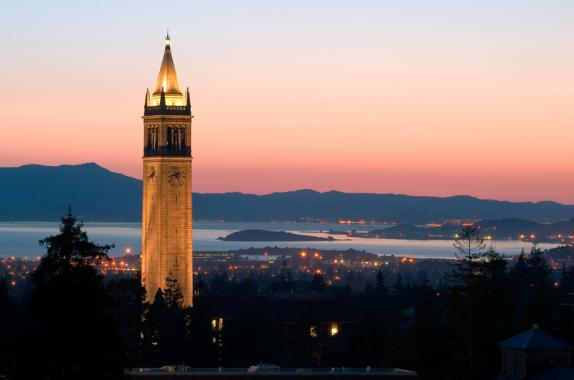
\includegraphics[width=1in]{campanile.jpg}				
	\end{subfigure}
	\begin{subfigure}[t]{1in}
		\centering
		\caption{Berkeley 2}\label{fig:2b}
		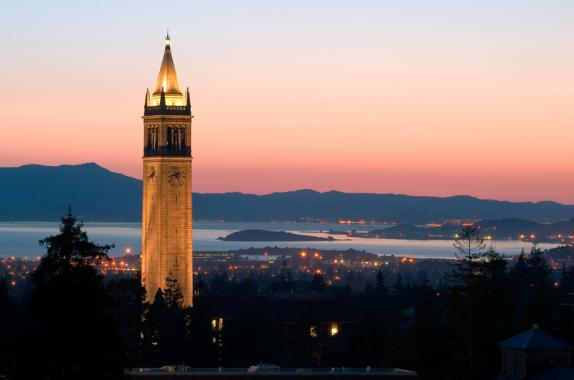
\includegraphics[width=1in]{campanile.jpg}		
	\end{subfigure}
	\caption{Berkeley at sunset - twice}\label{fig:2}
\end{figure}
\end{frame}

\end{document}